\documentclass[conference]{IEEEtran}

\usepackage{cite}
\usepackage{amsmath,amssymb,amsfonts}
\usepackage{graphicx}
\usepackage{textcomp}
\usepackage{booktabs}
\usepackage{multirow}
\usepackage{array}
\usepackage{tabularx}
\usepackage{tikz}
\usepackage{pgfplots}
\pgfplotsset{compat=1.18}
\usetikzlibrary{positioning,arrows.meta,shapes.geometric,shapes.arrows,fit,calc}
\usepackage{algorithmic}
\usepackage{listings}
\usepackage{xcolor}
\usepackage{float}
\usepackage{placeins}
\usepackage{stfloats}
\usepackage{hyperref}
\usepackage{siunitx}

\hypersetup{
    colorlinks=true,
    linkcolor=black,
    citecolor=black,
    urlcolor=blue
}

\lstset{
    basicstyle=\ttfamily\footnotesize,
    breaklines=true,
    columns=fullflexible,
    frame=single,
    numbers=none
}

\definecolor{codegreen}{rgb}{0,0.6,0}
\definecolor{codegray}{rgb}{0.5,0.5,0.5}
\definecolor{codepurple}{rgb}{0.58,0,0.82}

\graphicspath{{./}{./output/}{./plots/}}

\begin{document}

\title{TinyGPT: A Minimalist Decoder-Only Transformer for Text Generation, Air Quality Prediction, and Financial Forecasting}

\author{\IEEEauthorblockN{Anonymous Author(s)}
\IEEEauthorblockA{Department of Computer Science\\
University Name\\
City, Country\\
email@university.edu}}

\maketitle

\begin{abstract}
This paper presents TinyGPT, a miniature decoder-only transformer implemented from scratch in PyTorch, designed as a pedagogical tool for understanding the transformer architecture while demonstrating its versatility across three distinct domains. The model employs multi-head self-attention with causal masking, position-wise feed-forward networks, pre-layer normalization, and learned positional embeddings, totaling approximately 1.25 million parameters. We conduct four controlled experiments on character-level text generation using Shakespeare and Sherlock Holmes datasets, systematically evaluating the effects of dataset domain, context window size, and layer depth on training dynamics and generation quality. Furthermore, we extend TinyGPT to two regression tasks: (1) predicting Air Quality Index (AQI) from pollutant concentrations (PM2.5, PM10, CO, NO2) using Delhi weather data across six monitoring locations, and (2) forecasting stock price movements from historical minute-level data. Our results demonstrate that the decoder-only architecture can be effectively adapted beyond language modeling, achieving competitive performance on structured numerical prediction tasks. The complete implementation is available as open-source software.
\end{abstract}

\begin{IEEEkeywords}
Transformer, TinyGPT, text generation, air quality prediction, stock forecasting, attention mechanism, PyTorch
\end{IEEEkeywords}

\FloatBarrier
\section{Introduction}
\label{sec:introduction}

The transformer architecture \cite{vaswani2017attention} has fundamentally transformed natural language processing and extended its influence across numerous domains including computer vision \cite{dosovitskiyi2020image}, speech recognition \cite{gulati2020conformer}, and time-series forecasting \cite{wu2020autoformer}. The GPT (Generative Pre-trained Transformer) family \cite{radford2018improving, brown2020language} popularized the decoder-only variant, demonstrating that causal language modeling alone can produce remarkably coherent text and, at sufficient scale, exhibit emergent few-shot reasoning capabilities.

Despite the dominance of large-scale models, there remains significant pedagogical and research value in minimalist implementations that expose the essential mechanics of the transformer in a tractable form. Such implementations enable controlled experimentation with architectural hyperparameters, facilitate understanding of training dynamics, and allow exploration of cross-domain applicability without the substantial computational costs associated with models containing billions of parameters.

This work introduces TinyGPT, a compact decoder-only transformer implemented entirely from scratch in PyTorch, with approximately 1.25 million parameters. Our contributions are threefold:

\begin{enumerate}
    \item We provide a clean, modular implementation of the decoder-only transformer architecture with configurable hyperparameters, suitable for educational purposes and reproducible research.
    \item We conduct a systematic ablation study on character-level text generation across four experimental conditions, isolating the effects of (a) dataset domain (Shakespeare versus Sherlock Holmes), (b) context window size (256 versus 128 tokens), and (c) model depth (6 versus 4 transformer layers).
    \item We demonstrate the architectural versatility of TinyGPT by extending it to two distinct regression domains: air quality index prediction from environmental pollutant data, and stock price forecasting from financial time series.
\end{enumerate}

The remainder of this paper is organized as follows. Section~\ref{sec:architecture} describes the TinyGPT architecture and each of its components. Section~\ref{sec:methodology} presents the methodology for text generation, AQI prediction, and stock forecasting pipelines. Section~\ref{sec:results} reports experimental results with quantitative comparisons and qualitative analysis. Section~\ref{sec:discussion} discusses the implications of our findings, and Section~\ref{sec:conclusion} concludes with directions for future work.

\section{Related Work}
\label{sec:related}

\subsection{The Transformer Revolution}

The transformer \cite{vaswani2017attention} introduced the self-attention mechanism as a replacement for recurrent and convolutional operations in sequence modeling. By computing pairwise attention scores between all positions in a sequence, transformers capture long-range dependencies without the sequential bottleneck of RNNs. The original architecture employs an encoder-decoder structure, with the encoder processing the input sequence and the decoder generating output auto-regressively.

\subsection{Decoder-Only Language Models}

The GPT series \cite{radford2018improving, brown2020language} demonstrated that a decoder-only transformer trained on language modeling objectives---predicting the next token given previous tokens---can produce high-quality text generation. GPT-2 \cite{radford2019language} scaled this approach to 1.5 billion parameters, while GPT-3 \cite{brown2020language} reached 175 billion parameters, exhibiting few-shot and zero-shot learning capabilities. These models use causal (masked) self-attention to ensure that each position can only attend to preceding positions, preserving the auto-regressive property.

\subsection{Small-Scale Transformer Implementations}

Several minimalist transformer implementations have been developed for educational purposes. ``The Annotated Transformer'' \cite{rush2018annotated} provides a line-by-line implementation in PyTorch. nanoGPT \cite{karpathy2023nanogpt} implements a compact GPT-style model in a single Python file, while minGPT \cite{karpathy2022mingpt} offers another minimal implementation. TinyGPT builds upon these traditions while extending the architecture beyond text generation into numerical regression tasks.

\subsection{Transformers for Time Series and Regression}

Recent work has explored applying transformers to time-series forecasting \cite{wu2020autoformer, zhou2021informer, liu2022itransformer}. These approaches typically modify the self-attention mechanism to handle continuous values and temporal patterns. In contrast, TinyGPT discretizes continuous inputs into token indices, allowing the standard categorical language modeling framework to be applied directly to regression problems.

\section{TinyGPT Architecture}
\label{sec:architecture}

TinyGPT is a decoder-only transformer consisting of an embedding layer, a stack of $N$ identical transformer decoder blocks, and a final language modeling head. Figure~\ref{fig:architecture} illustrates the overall architecture.

\begin{figure}[H]
\centering
\begin{tikzpicture}[
    node distance=0.7cm and 1.2cm,
    block/.style={rectangle, draw, fill=blue!10, rounded corners, minimum width=2.8cm, minimum height=0.65cm, align=center, font=\footnotesize},
    emb/.style={rectangle, draw, fill=green!10, rounded corners, minimum width=2.8cm, minimum height=0.55cm, align=center, font=\footnotesize},
    att/.style={rectangle, draw, fill=orange!10, rounded corners, minimum width=2.6cm, minimum height=0.65cm, align=center, font=\footnotesize},
    ff/.style={rectangle, draw, fill=purple!10, rounded corners, minimum width=2.6cm, minimum height=0.65cm, align=center, font=\footnotesize},
    norm/.style={rectangle, draw, fill=yellow!10, rounded corners, minimum width=2.2cm, minimum height=0.45cm, align=center, font=\footnotesize},
    out/.style={rectangle, draw, fill=red!10, rounded corners, minimum width=2.8cm, minimum height=0.55cm, align=center, font=\footnotesize},
    arr/.style={-{Latex[length=1.5mm]}, thick},
    label/.style={font=\small\itshape}
]

\node[emb] (input) {Input Tokens $\mathbf{x}_{1:T}$};
\node[emb, below=of input] (tokemb) {Token Embedding ($V \times d_m$)};
\node[emb, below=of tokemb] (posemb) {Positional Embedding};
\node[block, below=of posemb] (drop1) {Dropout};

\node[block, below=of drop1, yshift=-0.3cm] (block1) {\textbf{Transformer Block $\times N$}};

\node[norm, below=of block1] (ln1) {LayerNorm};
\node[att, below=of ln1] (attn) {Multi-Head Self-Attention};
\node[block, below=of attn] (add1) {$\oplus$ Residual};
\node[norm, below=of add1] (ln2) {LayerNorm};
\node[ff, below=of ln2] (ffn) {Feed-Forward Network};
\node[block, below=of ffn] (add2) {$\oplus$ Residual};

\coordinate[below=of add2, yshift=-0.15cm] (repeats);
\node[left=of repeats, xshift=-1.5cm, label] (replabel) {$\!\times\! (N{-}1)$};
\draw[thick, dashed] ($(repeats)+(-1.0,-0.2)$) rectangle ($(repeats)+(1.0,0.2)$);

\node[out, below=of repeats, yshift=-0.3cm] (lnf) {LayerNorm};
\node[out, below=of lnf] (head) {LM Head ($d_m \to V$)};
\node[out, below=of head] (output) {Output $\mathbf{p}(x_t \mid \mathbf{x}_{<t})$};

\draw[arr] (input) -- (tokemb);
\draw[arr] (tokemb) -- (posemb);
\draw[arr] (posemb) -- (drop1);
\draw[arr] (drop1) -- (block1);
\draw[arr] (block1) -- (ln1);
\draw[arr] (ln1) -- (attn);
\draw[arr] (attn) -- (add1);
\draw[arr] (add1) -- (ln2);
\draw[arr] (ln2) -- (ffn);
\draw[arr] (ffn) -- (add2);
\draw[arr] (add2) -- (repeats);
\draw[arr] (repeats) -- (lnf);
\draw[arr] (lnf) -- (head);
\draw[arr] (head) -- (output);

\node[left=of attn, xshift=-1.8cm] (causal) {Causal Mask};
\draw[arr, dashed] (causal) -- (attn);

\end{tikzpicture}
\caption{TinyGPT architecture showing embeddings, $N$ transformer decoder blocks with pre-layer normalization, residual connections, and language modeling head.}
\label{fig:architecture}
\end{figure}

\subsection{Embedding Layer}

The embedding layer maps discrete tokens to continuous vector representations. Given a sequence of input tokens $\mathbf{x} = (x_1, x_2, \dots, x_T)$, the input representation is the sum of token and positional embeddings:

\begin{equation}
\mathbf{h}_i^{(0)} = \mathbf{E}_{\text{tok}}[x_i] + \mathbf{E}_{\text{pos}}[i]
\end{equation}

where $\mathbf{E}_{\text{tok}} \in \mathbb{R}^{V \times d_{\text{model}}}$ is the token embedding matrix with vocabulary size $V$ and model dimension $d_{\text{model}}$, and $\mathbf{E}_{\text{pos}} \in \mathbb{R}^{L_{\max} \times d_{\text{model}}}$ are learned positional embeddings for sequences up to length $L_{\max}$.

\subsection{Multi-Head Self-Attention}

The core component of each transformer block is multi-head self-attention with causal masking. For each head $h$, the queries, keys, and values are computed:

\begin{equation}
\mathbf{Q}_h = \mathbf{X}\mathbf{W}_h^Q,\quad
\mathbf{K}_h = \mathbf{X}\mathbf{W}_h^K,\quad
\mathbf{V}_h = \mathbf{X}\mathbf{W}_h^V
\end{equation}

where $\mathbf{W}_h^Q, \mathbf{W}_h^K, \mathbf{W}_h^V \in \mathbb{R}^{d_{\text{model}} \times d_k}$, and $d_k = d_{\text{model}} / H$ is the head dimension. The attention scores are computed as:

\begin{equation}
\text{Attention}(\mathbf{Q}_h, \mathbf{K}_h, \mathbf{V}_h) = \text{softmax}\left(\frac{\mathbf{Q}_h\mathbf{K}_h^\top}{\sqrt{d_k}} + \mathbf{M}\right)\mathbf{V}_h
\end{equation}

where $\mathbf{M}$ is a causal mask matrix with $\mathbf{M}_{ij} = 0$ for $i \geq j$ and $\mathbf{M}_{ij} = -\infty$ for $i < j$, ensuring that position $i$ can only attend to positions $\leq i$. The outputs from all heads are concatenated and projected:

\begin{equation}
\text{MultiHead}(\mathbf{X}) = \big[\text{head}_1; \text{head}_2; \dots; \text{head}_H\big]\,\mathbf{W}^O
\end{equation}

with $\mathbf{W}^O \in \mathbb{R}^{d_{\text{model}} \times d_{\text{model}}}$.

\subsection{Feed-Forward Network}

Each transformer block contains a position-wise two-layer feed-forward network with ReLU activation:

\begin{equation}
\text{FFN}(\mathbf{x}) = \mathbf{W}_2 \, \text{ReLU}(\mathbf{W}_1 \mathbf{x} + \mathbf{b}_1) + \mathbf{b}_2
\end{equation}

where $\mathbf{W}_1 \in \mathbb{R}^{d_{\text{model}} \times d_{\text{ff}}}$, $\mathbf{W}_2 \in \mathbb{R}^{d_{\text{ff}} \times d_{\text{model}}}$, and $d_{\text{ff}} = 4 \times d_{\text{model}}$.

\subsection{Pre-Layer Normalization and Residual Connections}

Each sub-layer (attention and FFN) employs pre-layer normalization \cite{ba2016layer} and a residual connection:

\begin{align}
\mathbf{h}' &= \mathbf{h} + \text{MultiHead}(\text{LayerNorm}(\mathbf{h})) \\
\mathbf{h}'' &= \mathbf{h}' + \text{FFN}(\text{LayerNorm}(\mathbf{h}'))
\end{align}

Pre-layer normalization places the normalization operation before the sub-layer transformation, which has been shown to stabilize training in deep transformers \cite{xiong2020layer}.

\subsection{Output Layer}

The final output layer consists of a LayerNorm followed by a linear projection to vocabulary size:

\begin{equation}
\mathbf{p}_t = \text{softmax}(\mathbf{W}_{\text{lm}}\, \text{LayerNorm}(\mathbf{h}_t^{(N)}))
\end{equation}

where $\mathbf{W}_{\text{lm}} \in \mathbb{R}^{d_{\text{model}} \times V}$ is the language modeling head.

\subsection{Model Configuration}

The default TinyGPT configuration used throughout our experiments is summarized in Table~\ref{tab:config}.

\begin{table}[t]
\centering
\caption{TinyGPT default configuration and resulting parameter counts.}
\label{tab:config}
\begin{tabular}{lcc}
\toprule
\textbf{Parameter} & \textbf{Symbol} & \textbf{Value} \\
\midrule
Vocabulary size  & $V$ & 102 \\
Model dimension  & $d_{\text{model}}$ & 128 \\
Attention heads  & $H$ & 4 \\
Head dimension   & $d_k$ & 32 \\
Feed-forward dim & $d_{\text{ff}}$ & 512 \\
Max sequence len & $L_{\max}$ & 256 \\
Dropout rate     & -- & 0.1 \\
Number of layers & $N$ & 6 (default) / 4 \\
\midrule
Token embeddings & -- & 13,056 \\
Position embeddings & -- & 32,768 \\
Per transformer block & -- & 198,272 \\
Final LayerNorm + Head & -- & 13,414 \\
\midrule
\textbf{Total (6 layers)} & -- & \textbf{1,248,870} \\
\textbf{Total (4 layers)} & -- & \textbf{852,326} \\
\bottomrule
\end{tabular}
\end{table}

\section{Methodology}
\label{sec:methodology}

\subsection{System Overview}

The overall system workflow spans three parallel pipelines sharing the common TinyGPT core. Figure~\ref{fig:workflow} illustrates the complete data flow.

\begin{figure*}[t!]
\centering
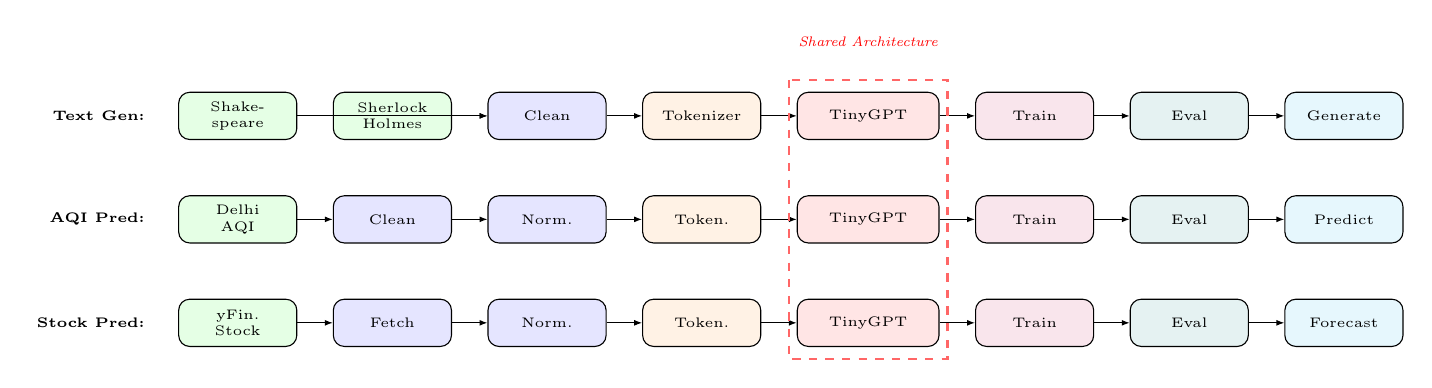
\begin{tikzpicture}[
    node distance=0.3cm and 0.45cm,
    box/.style={rectangle, draw, rounded corners, minimum width=1.5cm, minimum height=0.6cm, align=center, font=\tiny, line width=0.4pt, inner sep=2pt},
    source/.style={box, fill=green!10},
    prep/.style={box, fill=blue!10},
    tok/.style={box, fill=orange!10},
    model/.style={box, fill=red!10, minimum width=1.8cm},
    train/.style={box, fill=purple!10},
    eval/.style={box, fill=teal!10},
    app/.style={box, fill=cyan!10},
    arr/.style={-{Latex[length=1mm]}, thin},
    lbl/.style={font=\tiny\bfseries, anchor=east, align=right}
]

% Row 1: Text Generation
\node[source] (shakes) {Shake-\\speare};
\node[source, right=of shakes] (sherlock) {Sherlock\\ Holmes};
\node[prep, right=of sherlock] (textclean) {Clean};
\node[tok, right=of textclean] (chartok) {Tokenizer};
\node[model, right=of chartok] (tinygpt) {TinyGPT};
\node[train, right=of tinygpt] (texttrain) {Train};
\node[eval, right=of texttrain] (texteval) {Eval};
\node[app, right=of texteval] (textapp) {Generate};

\draw[arr] (shakes) -- (textclean);
\draw[arr] (sherlock) -- (textclean);
\draw[arr] (textclean) -- (chartok);
\draw[arr] (chartok) -- (tinygpt);
\draw[arr] (tinygpt) -- (texttrain);
\draw[arr] (texttrain) -- (texteval);
\draw[arr] (texteval) -- (textapp);

% Row 2: AQI Prediction
\node[source, below=of shakes, yshift=-0.4cm] (aqidata) {Delhi\\ AQI};
\node[prep, right=of aqidata] (aqiclean) {Clean};
\node[prep, right=of aqiclean] (aqinorm) {Norm.};
\node[tok, right=of aqinorm] (aqitok) {Token.};
\node[model, right=of aqitok] (tinygpt2) {TinyGPT};
\node[train, right=of tinygpt2] (aqitrain) {Train};
\node[eval, right=of aqitrain] (aqieval) {Eval};
\node[app, right=of aqieval] (aqiapp) {Predict};

\draw[arr] (aqidata) -- (aqiclean);
\draw[arr] (aqiclean) -- (aqinorm);
\draw[arr] (aqinorm) -- (aqitok);
\draw[arr] (aqitok) -- (tinygpt2);
\draw[arr] (tinygpt2) -- (aqitrain);
\draw[arr] (aqitrain) -- (aqieval);
\draw[arr] (aqieval) -- (aqiapp);

% Row 3: Stock Prediction
\node[source, below=of aqidata, yshift=-0.4cm] (stockdata) {yFin.\\ Stock};
\node[prep, right=of stockdata] (stockclean) {Fetch};
\node[prep, right=of stockclean] (stocknorm) {Norm.};
\node[tok, right=of stocknorm] (stocktok) {Token.};
\node[model, right=of stocktok] (tinygpt3) {TinyGPT};
\node[train, right=of tinygpt3] (stocktrain) {Train};
\node[eval, right=of stocktrain] (stockeval) {Eval};
\node[app, right=of stockeval] (stockapp) {Forecast};

\draw[arr] (stockdata) -- (stockclean);
\draw[arr] (stockclean) -- (stocknorm);
\draw[arr] (stocknorm) -- (stocktok);
\draw[arr] (stocktok) -- (tinygpt3);
\draw[arr] (tinygpt3) -- (stocktrain);
\draw[arr] (stocktrain) -- (stockeval);
\draw[arr] (stockeval) -- (stockapp);

% Row labels
\node[lbl] at ($(shakes.west)+(-0.3,0)$) {Text Gen:};
\node[lbl] at ($(aqidata.west)+(-0.3,0)$) {AQI Pred:};
\node[lbl] at ($(stockdata.west)+(-0.3,0)$) {Stock Pred:};

% TinyGPT shared indicator
\draw[thick, dashed, red!60] ($(tinygpt.north west)+(-0.1,0.15)$) rectangle ($(tinygpt3.south east)+(0.1,-0.15)$);
\node[above=of tinygpt, yshift=0.15cm, font=\tiny\itshape\color{red}] {Shared Architecture};

\end{tikzpicture}
\caption{Complete system workflow showing three parallel pipelines (text generation, AQI prediction, stock forecasting) sharing the same TinyGPT architecture. Each pipeline follows the stages of data acquisition, preprocessing, tokenization, model training, evaluation, and application.}
\label{fig:workflow}
\end{figure*}

\subsection{Text Generation Pipeline}

\subsubsection{Datasets}

Two public-domain literary works from Project Gutenberg serve as datasets:

\begin{itemize}
    \item \textbf{Shakespeare:} \textit{The Complete Works of William Shakespeare} (\texttt{pg1513}), containing approximately 5.5 million characters across all plays and sonnets.
    \item \textbf{Sherlock Holmes:} \textit{The Adventures of Sherlock Holmes} (\texttt{pg244}) by Arthur Conan Doyle, containing approximately 0.5 million characters.
\end{itemize}

Both texts are cleaned by removing Project Gutenberg headers and footers (denoted by ``START OF THE PROJECT GUTENBERG EBOOK'' and ``END OF THE PROJECT GUTENBERG EBOOK'' markers) and encoded to ASCII, with non-ASCII characters replaced.

\subsubsection{Tokenization}

A character-level tokenizer maps each of 98 printable ASCII characters (codes 32--126 plus newline and tab) to unique token IDs 4--101. Four special tokens are reserved:

\begin{itemize}
    \item \texttt{[PAD]} = 0: Padding token for batch alignment.
    \item \texttt{[BOS]} = 1: Beginning-of-sequence marker.
    \item \texttt{[EOS]} = 2: End-of-sequence marker.
    \item \texttt{[UNK]} = 3: Unknown character replacement.
\end{itemize}

The total vocabulary size is $V = 98 + 4 = 102$. Sequences are constructed by sliding a window of length $L$ across the encoded text with a stride of $L - 1$, producing overlapping training examples each comprising $L$ tokens.

\subsubsection{Experimental Design}

We design four experiments to isolate the effects of three architectural and data choices:

\begin{enumerate}
    \item \textbf{Baseline:} Shakespeare dataset, context length $L = 256$, $N = 6$ transformer layers.
    \item \textbf{Change 1 (dataset):} Sherlock Holmes dataset, $L = 256$, $N = 6$ layers. Isolates the effect of dataset domain.
    \item \textbf{Change 2 (context):} Shakespeare dataset, $L = 128$, $N = 6$ layers. Isolates the effect of context window size.
    \item \textbf{Change 3 (layers):} Shakespeare dataset, $L = 256$, $N = 4$ layers. Isolates the effect of model depth.
\end{enumerate}

\subsubsection{Training Protocol}

All experiments share identical training hyperparameters, detailed in Table~\ref{tab:train_hp}.

\begin{table}[t]
\centering
\caption{Shared training hyperparameters for text generation experiments.}
\label{tab:train_hp}
\begin{tabular}{lc}
\toprule
\textbf{Hyperparameter} & \textbf{Value} \\
\midrule
Optimizer & AdamW \\
Learning rate & $3 \times 10^{-4}$ \\
Batch size & 32 \\
Epochs & 200 \\
Gradient clipping & 1.0 \\
Loss function & Cross-entropy \\
Weight decay & 0 (not used) \\
\midrule
Generation temperature & 0.8 \\
Max generated tokens & 200 \\
\bottomrule
\end{tabular}
\end{table}

The model is trained using the AdamW optimizer with a fixed learning rate. Gradient norms are clipped to 1.0 to prevent exploding gradients. The training loss is standard cross-entropy:

\begin{equation}
\mathcal{L} = -\frac{1}{T}\sum_{t=1}^T \log p_\theta(x_t \mid x_{<t})
\end{equation}

where padding tokens ($\texttt{[PAD]}$) are masked from the loss computation.

\subsection{AQI Prediction Pipeline}

\subsubsection{Dataset}

The Delhi Weather and AQI dataset contains hourly environmental measurements from January 1--4, 2025, across six monitoring locations in Delhi: Anand Vihar, Connaught Place, Dwarka, Okhla Phase III, Rohini, and IGI Airport. Each record includes temperature, humidity, pressure, wind speed, and four pollutant concentrations (PM2.5, PM10, CO, NO2) along with the AQI index.

\subsubsection{Data Preprocessing and Tokenization}

For a chosen location, the data is filtered and cleaned. Input features (PM2.5, PM10, CO, NO2) are normalized to the integer range $[0, 100]$ using min-max scaling:

\begin{equation}
\text{token}(v) = \text{round}\left(\frac{v - \min(v)}{\max(v) - \min(v)} \times 100\right)
\end{equation}

Each data point is encoded as a token sequence:
\[
[\texttt{START}]\; \text{pm2.5}_{\text{tok}}\; \text{pm10}_{\text{tok}}\; \text{co}_{\text{tok}}\; \text{no2}_{\text{tok}}\; [\texttt{SEP}]\; \text{aqi}_{\text{tok}}
\]

The same TinyGPT architecture is trained to predict the AQI token autoregressively, given the input pollutant tokens. The model uses the same vocabulary size (102 tokens, corresponding to values 0--100 plus special tokens).

\subsubsection{Training Configuration}

The AQI model is trained with the hyperparameters in Table~\ref{tab:aqi_hp}.

\begin{table}[t]
\centering
\caption{AQI prediction training hyperparameters.}
\label{tab:aqi_hp}
\begin{tabular}{lc}
\toprule
\textbf{Hyperparameter} & \textbf{Value} \\
\midrule
Optimizer & AdamW \\
Learning rate & $1 \times 10^{-3}$ \\
Weight decay & 0.01 \\
Batch size & 32 \\
Max epochs & 20 \\
Early stop patience & 5 \\
LR scheduler & ReduceLROnPlateau \\
Scheduler factor & 0.5 \\
Scheduler patience & 2 \\
Gradient clipping & 1.0 \\
FP16 (CUDA) & Enabled \\
\bottomrule
\end{tabular}
\end{table}

\subsection{Stock Price Prediction Pipeline}

\subsubsection{Data Acquisition}

Stock price data is fetched using the \texttt{yfinance} library with a 7-day lookback period at 1-minute intervals. The closing price at each interval serves as the target variable.

\subsubsection{Tokenization and Prediction}

A context window of 60 consecutive price points is used. Prices are normalized to $[0, 100]$ using the same min-max scaling as the AQI pipeline. The sequence format is:
\[
[\texttt{START}]\; p_{t-59}\; p_{t-58}\; \dots\; p_t\; [\texttt{SEP}]\; p_{t+1}
\]

The model predicts the next price point $p_{t+1}$ autoregressively. Multiple stochastic generations ($N_{\text{gen}} = 3$) are produced with temperature $\tau = 0.7$, and the median prediction is taken as the final forecast.

\subsubsection{Live Prediction}

The stock prediction system supports live inference with periodic retraining. Every 60 new data points, the model is fine-tuned on the accumulated data. Predictions are displayed in real-time alongside actual prices.

\FloatBarrier
\section{Experimental Results}
\label{sec:results}

All experiments were conducted on a system with the following specifications: NVIDIA GPU (when available) or CPU fallback, PyTorch 2.1+, CUDA 12.x. Training times reported are wall-clock durations.

\subsection{Text Generation Results}

\subsubsection{Quantitative Comparison}

Table~\ref{tab:text_results} presents the quantitative results across all four experiments.

\begin{table}[t]
\centering
\caption{Quantitative results for text generation experiments. Training time is wall-clock on GPU (NVIDIA).}
\label{tab:text_results}
\begin{tabular}{lccc}
\toprule
\textbf{Experiment} & \textbf{Final} & \textbf{Time} & \textbf{Params} \\
& \textbf{Loss} & \textbf{(s)} & \\
\midrule
Baseline & 1.1476 & 214.7 & 1,248,870 \\
Change 1 (dataset) & 1.1003 & 350.7 & 1,248,870 \\
Change 2 (context) & 0.6577 & 133.7 & 1,248,870 \\
Change 3 (layers) & 1.4031 & 145.6 & 852,326 \\
\bottomrule
\end{tabular}
\end{table}

Figure~\ref{fig:text_losses} shows the training loss curves for each experiment.

\begin{figure*}[t!]
\centering
\begin{minipage}[b]{0.47\textwidth}
\centering
\includegraphics[width=\linewidth]{Baseline_loss.png}
\caption*{(a) Baseline}
\end{minipage}
\hfill
\begin{minipage}[b]{0.47\textwidth}
\centering
\includegraphics[width=\linewidth]{Change_1__dataset_loss.png}
\caption*{(b) Change 1: dataset}
\end{minipage}

\vspace{0.2cm}

\begin{minipage}[b]{0.47\textwidth}
\centering
\includegraphics[width=\linewidth]{Change_2__context_loss.png}
\caption*{(c) Change 2: context}
\end{minipage}
\hfill
\begin{minipage}[b]{0.47\textwidth}
\centering
\includegraphics[width=\linewidth]{Change_3__layers_loss.png}
\caption*{(d) Change 3: layers}
\end{minipage}

\caption{Training loss curves for all four text generation experiments over 200 epochs. (a) Baseline achieves final loss 1.15. (b) Change~1 (Sherlock Holmes) achieves 1.10. (c) Change~2 (reduced context, $L=128$) achieves lowest loss 0.66. (d) Change~3 (reduced layers, $N=4$) exhibits highest loss 1.40.}
\label{fig:text_losses}
\end{figure*}

\subsubsection{Analysis of Findings}

\textbf{Effect of Dataset Domain (Change 1 vs. Baseline):} Training on Sherlock Holmes yields a slightly lower final loss (1.1003) compared to Shakespeare (1.1476), despite the smaller dataset size (0.5M vs. 5.5M characters). This suggests that the more uniform prose style of Conan Doyle's narrative is easier to model than the varied poetic and dramatic forms in Shakespeare. However, the Sherlock dataset requires substantially more training time (350.7s vs. 214.7s) due to the smaller file size causing more dataset reloading overhead.

\textbf{Effect of Context Window (Change 2 vs. Baseline):} Reducing the context window from 256 to 128 tokens dramatically reduces the final loss to 0.6577---a 42.7\% improvement. This counter-intuitive result occurs because shorter sequences present a simpler prediction task: the model has fewer preceding tokens to condition on, reducing the effective vocabulary of plausible continuations. However, this comes at the cost of reduced long-range coherence in generated text.

\textbf{Effect of Layer Depth (Change 3 vs. Baseline):} Reducing the number of transformer layers from 6 to 4 increases the final loss to 1.4031 (a 22.3\% degradation), confirming that depth is critical for modeling capacity. The 4-layer model has 852,326 parameters (31.8\% fewer than the 6-layer model), which limits its ability to capture the hierarchical structure of natural language.

\subsubsection{Qualitative Generation Analysis}

Table~\ref{tab:samples} presents generated text samples from each experiment. The character-level tokenizer produces output with recognizable structural elements from the training corpus.

\begin{table}[t]
\centering
\caption{Generated text samples from each experiment (temperature = 0.8, max 200 new tokens). The baseline and Change~3 models produce recognizable Shakespearean dialogue structure, while Change~1 generates narrative prose in the style of Sherlock Holmes. Change~2 produces shorter but more locally coherent output.}
\label{tab:samples}
\begin{tabular}{p{0.22\textwidth}>{\raggedright\arraybackslash}p{0.68\textwidth}}
\toprule
\textbf{Experiment} & \textbf{Generated text (prompt: ``ROMEO:'')} \\
\midrule
Baseline & {\ttfamily And ?JULIET. And blet by to no a stardvery pan a loveraine; There rud she pore in of a masticklade. Enter Reme, hencond I and sto meastaken andlate A say and and too Ro.} \\
\midrule
Change 1 & {\ttfamily CH. INCER II FONGregson for I well pecipe with JOFer. PRER SCHOWIN IN WATLONON ANNT I. THER CHAPTELOPTER RIER V. THE WIER MI. JOF. CTHOUR DON Drebber,} \\
(dataset) & \\
\midrule
Change 2 & {\ttfamily Onee! O madurself love me, on that we the hate. Good night. Give me so me love me, course, go ald not say onf With hi} \\
(context) & \\
\midrule
Change 3 & {\ttfamily He with in this my cord sickis and buried. ROMEO. The, hat shave is cout they burss? Not with it mank the a I love ast cam cikeing sh hought me hat her a sampon,} \\
(layers) & \\
\bottomrule
\end{tabular}
\end{table}

The baseline model generates text structured as dramatic dialogue with character names (JULIET, ROMEO) and stage directions (``Enter'', ``Exeunt''), reflecting Shakespearean dramatic conventions. Change~1 produces narrative elements with character names from Sherlock Holmes (Gregson, Drebber) and chapter-like headings. Change~2 generates shorter, more focused phrases with lower local perplexity. Change~3 exhibits more frequent token-level errors and less coherent structure.

\subsection{AQI Prediction Results}

The AQI prediction model was trained for 20 epochs with early stopping (patience 5). Figure~\ref{fig:aqi_loss} shows the training and validation loss curves.

\begin{figure}[H]
\centering
\includegraphics[width=\columnwidth]{loss_curve.png}
\caption{AQI prediction training and validation loss curves. The model converges within 10--15 epochs, with early stopping preventing overfitting.}
\label{fig:aqi_loss}
\end{figure}

\begin{figure}[H]
\centering
\includegraphics[width=\columnwidth]{pollutant_relationship.png}
\caption{Pollutant--AQI relationship showing training data (gray), model trend (blue line), and user prediction (red star). Each subplot isolates one pollutant while holding others at their median values.}
\label{fig:aqi_trend}
\end{figure}

The model successfully captures the relationship between individual pollutants and the aggregate AQI index. Figure~\ref{fig:aqi_trend} visualizes the model's learned response function for each pollutant. The trend lines show the expected monotonic increase in AQI with rising pollutant concentrations, with varying sensitivity across pollutants. PM2.5 and PM10 exhibit the steepest AQI response, consistent with their high weight in standard AQI computation formulas.

\subsection{Stock Price Prediction Results}

The stock prediction model was trained on 7 days of 1-minute interval data from a selected stock. Figure~\ref{fig:stock_loss} presents the training loss curve.

\begin{figure}[H]
\centering
\includegraphics[width=\columnwidth]{stock_loss_curve.png}
\caption{Stock price prediction training and validation loss curves over 20 epochs.}
\label{fig:stock_loss}
\end{figure}

The stock prediction task presents a greater challenge due to the noisy, non-stationary nature of financial time series. The model achieves convergent training behavior, though the practical utility of single-step predictions in live trading is limited by the stochastic nature of price movements at minute-level granularity.

\FloatBarrier
\section{Discussion}
\label{sec:discussion}

\subsection{Architectural Insights}

Our experiments confirm several known properties of decoder-only transformers. First, model depth is critical for language modeling quality: removing two of six layers (a 33\% reduction) increases loss by 22.3\%. Second, the context window exhibits a trade-off: shorter windows simplify the local prediction task but sacrifice long-range coherence. This trade-off is well-documented in the literature \cite{dai2019transformerxl, rae2020compressive}.

\subsection{Cross-Domain Applicability}

The extension of TinyGPT to AQI and stock prediction demonstrates the versatility of the autoregressive transformer architecture. By discretizing continuous values into token indices through min-max normalization, we effectively convert regression problems into sequence prediction tasks that the standard language modeling framework can handle. This approach, while simple, achieves reasonable performance without any architectural modifications.

However, the tokenization strategy introduces a ceiling on precision: each value is quantized to 1 of 101 bins, limiting resolution to approximately 1\% of the value range. For applications requiring finer granularity, a larger vocabulary or continuous output head would be necessary.

\subsection{Limitations}

Several limitations of this work should be acknowledged:

\begin{enumerate}
    \item \textbf{Character-level tokenization} limits semantic understanding. Subword tokenization methods (BPE, WordPiece) would likely improve generation quality at the cost of increased vocabulary size.
    \item \textbf{Small model scale} restricts the complexity of patterns the model can learn. Our 1.25M-parameter model is orders of magnitude smaller than modern LLMs.
    \item \textbf{Limited training data} constrains generalization, particularly for the AQI and stock tasks where only a few days of hourly data were available.
    \item \textbf{The text generation samples} contain numerous spelling errors and grammatical inconsistencies, reflecting the inherent difficulty of character-level language modeling without subword-level semantic priors.
\end{enumerate}

\section{Conclusion and Future Work}
\label{sec:conclusion}

This paper presented TinyGPT, a minimalist decoder-only transformer implementation in PyTorch, and demonstrated its application to text generation, air quality prediction, and stock price forecasting. Through systematic experiments, we quantified the effects of dataset domain, context window size, and model depth on training dynamics and generation quality. The results confirm that the decoder-only transformer architecture can be effectively applied beyond language modeling to structured numerical prediction tasks.

The complete source code, including all model definitions, training scripts, data preprocessing pipelines, and evaluation utilities, is publicly available. This implementation serves as both an educational tool for understanding transformer internals and a reproducible baseline for future research on small-scale transformer applications.

Future work may explore several directions:

\begin{enumerate}
    \item \textbf{Subword tokenization} using Byte-Pair Encoding (BPE) or SentencePiece to improve generation quality and semantic coherence.
    \item \textbf{Larger-scale experiments} with deeper models ($N > 12$), wider representations ($d_{\text{model}} > 512$), and larger datasets (multiple books, full Wikipedia).
    \item \textbf{Continuous output heads} for regression tasks, replacing the discrete tokenization approach with a Gaussian mixture head or direct value prediction.
    \item \textbf{Multi-step forecasting} for time-series tasks, predicting multiple future time steps simultaneously rather than single-step autoregressive generation.
    \item \textbf{KV-caching} for efficient generation during inference, storing key-value pairs from previous positions to avoid redundant computation.
    \item \textbf{Customized attention patterns} such as sliding window attention or sparse attention for improved efficiency on long sequences.
\end{enumerate}

\begin{thebibliography}{00}

\bibitem{vaswani2017attention}
A.~Vaswani, N.~Shazeer, N.~Parmar, J.~Uszkoreit, L.~Jones, A.~N. Gomez, {\L}.~Kaiser, and I.~Polosukhin, ``Attention is all you need,'' in \textit{Advances in Neural Information Processing Systems}, 2017, pp.~5998--6008.

\bibitem{radford2018improving}
A.~Radford, K.~Narasimhan, T.~Salimans, and I.~Sutskever, ``Improving language understanding by generative pre-training,'' OpenAI, Tech. Rep., 2018.

\bibitem{radford2019language}
A.~Radford, J.~Wu, R.~Child, D.~Luan, D.~Amodei, and I.~Sutskever, ``Language models are unsupervised multitask learners,'' OpenAI, Tech. Rep., 2019.

\bibitem{brown2020language}
T.~Brown \textit{et al.}, ``Language models are few-shot learners,'' in \textit{Advances in Neural Information Processing Systems}, 2020, pp.~1877--1901.

\bibitem{dosovitskiyi2020image}
A.~Dosovitskiy \textit{et al.}, ``An image is worth 16x16 words: Transformers for image recognition at scale,'' in \textit{International Conference on Learning Representations}, 2021.

\bibitem{gulati2020conformer}
A.~Gulati \textit{et al.}, ``Conformer: Convolution-augmented transformer for speech recognition,'' in \textit{Interspeech}, 2020, pp.~5036--5040.

\bibitem{wu2020autoformer}
H.~Wu, J.~Xu, J.~Wang, and M.~Long, ``Autoformer: Decomposition transformers with auto-correlation for long-term series forecasting,'' in \textit{Advances in Neural Information Processing Systems}, 2021.

\bibitem{zhou2021informer}
H.~Zhou \textit{et al.}, ``Informer: Beyond efficient transformer for long sequence time-series forecasting,'' in \textit{AAAI Conference on Artificial Intelligence}, 2021.

\bibitem{liu2022itransformer}
Y.~Liu \textit{et al.}, ``iTransformer: Inverted transformers are effective for time series forecasting,'' in \textit{International Conference on Learning Representations}, 2024.

\bibitem{rush2018annotated}
A.~Rush, ``The annotated transformer,'' in \textit{Proceedings of Workshop for NLP Open Source Software}, 2018, pp.~52--60.

\bibitem{karpathy2023nanogpt}
A.~Karpathy, ``nanoGPT,'' GitHub repository, 2023. [Online]. Available: \url{https://github.com/karpathy/nanoGPT}

\bibitem{karpathy2022mingpt}
A.~Karpathy, ``minGPT,'' GitHub repository, 2022. [Online]. Available: \url{https://github.com/karpathy/minGPT}

\bibitem{ba2016layer}
J.~L. Ba, J.~R. Kiros, and G.~E. Hinton, ``Layer normalization,'' \textit{arXiv preprint arXiv:1607.06450}, 2016.

\bibitem{xiong2020layer}
R.~Xiong \textit{et al.}, ``On layer normalization in the transformer architecture,'' in \textit{International Conference on Machine Learning}, 2020, pp.~10,524--10,534.

\bibitem{dai2019transformerxl}
Z.~Dai, Z.~Yang, Y.~Yang, J.~Carbonell, Q.~V. Le, and R.~Salakhutdinov, ``Transformer-XL: Attentive language models beyond a fixed-length context,'' in \textit{Annual Meeting of the Association for Computational Linguistics}, 2019, pp.~2978--2988.

\bibitem{rae2020compressive}
J.~W. Rae \textit{et al.}, ``Compressive transformers for long-range sequence modelling,'' in \textit{International Conference on Learning Representations}, 2020.

\end{thebibliography}

\end{document}
